%% (Master) Thesis template
% Template version used: v1.4
%
% Largely adapted from Adrian Nievergelt's template for the ADPS
% (lecture notes) project.


%% We use the memoir class because it offers a many easy to use features.
\documentclass[11pt,a4paper,titlepage]{memoir}

%% Packages
%% ========

%% LaTeX Font encoding -- DO NOT CHANGE
\usepackage[OT1]{fontenc}

%% Babel provides support for languages.  'english' uses British
%% English hyphenation and text snippets like "Figure" and
%% "Theorem". Use the option 'ngerman' if your document is in German.
%% Use 'american' for American English.  Note that if you change this,
%% the next LaTeX run may show spurious errors.  Simply run it again.
%% If they persist, remove the .aux file and try again.
\usepackage[english]{babel}

%% Input encoding 'utf8'. In some cases you might need 'utf8x' for
%% extra symbols. Not all editors, especially on Windows, are UTF-8
%% capable, so you may want to use 'latin1' instead.
\usepackage[utf8]{inputenc}

%% This changes default fonts for both text and math mode to use Herman Zapfs
%% excellent Palatino font.  Do not change this.
\usepackage[sc]{mathpazo}

%% The AMS-LaTeX extensions for mathematical typesetting.  Do not
%% remove.
\usepackage{amsmath,amssymb,amsfonts,mathrsfs}

%% NTheorem is a reimplementation of the AMS Theorem package. This
%% will allow us to typeset theorems like examples, proofs and
%% similar.  Do not remove.
%% NOTE: Must be loaded AFTER amsmath, or the \qed placement will
%% break
\usepackage[amsmath,thmmarks]{ntheorem}

%% LaTeX' own graphics handling
\usepackage{graphicx}


%% This allows you to add .pdf files. It is used to add the
%% declaration of originality.
\usepackage{pdfpages}


%% Our layout configuration.  DO NOT CHANGE.
\input{layoutsetup}

%% Theorem environments.  You will have to adapt this for a German
%% thesis.
\input{theoremsetup}


%% Make document internal hyperlinks wherever possible. (TOC, references)
%% This MUST be loaded after varioref, which is loaded in 'extrapackages'
%% above.  We just load it last to be safe.
\usepackage[linkcolor=black,colorlinks=true,citecolor=black,filecolor=black]{hyperref}

%% This allows you to use "\cref{sec:your-section}" instead of writing out 
%% "Section~\ref{sec:your-section}", also works for tables, figures, etc.
%% Use \Cref at the beginning of a sentence and \cref elsewhere.
%% Must be loaded after hyperref.
\usepackage[capitalise]{cleveref}

%% TikZ for diagrams
\usepackage{tikz}
\usetikzlibrary{shapes.geometric, positioning, arrows.meta, calc}

%% Package for TODO notes
\usepackage{todonotes}

%% For figure positioning
\usepackage{float}

%% For plots
\usepackage{pgfplots}
% For better tables
\usepackage{booktabs}
\usepackage{multirow}
% For mathematical symbols
\usepackage{amsmath}

%% Document information
%% ====================

\title{Secure and Private Web Proxy with TEE Support}
\author{Riccardo Negri}
\thesistype{Master's Semester Project}
\advisors{Professor: Prof. Dr. Srdjan Capkun\\
Supervisors: Dr. Yoshimichi Nakatsuka}
\department{System Security Group\\Institute of Information Security\\Department of Computer Science}
\date{September 11, 2024}

\begin{document}

\frontmatter

%% Title page is autogenerated from document information above.  DO
%% NOT CHANGE.
\begin{titlingpage}
  \calccentering{\unitlength}
  \begin{adjustwidth*}{\unitlength-24pt}{-\unitlength-24pt}
    \maketitle
  \end{adjustwidth*}
\end{titlingpage}

%% The abstract of your thesis.  Edit the file as needed.
\begin{abstract}
Web proxy services are critical tools that allow users to access web content otherwise restricted by geographical or technological barriers. However, these services introduce significant security and privacy risks, as highlighted by research exposing vulnerabilities such as man-in-the-middle attacks, credential theft, and session hijacking. These risks primarily stem from the need to trust the service operators. This project explores the feasibility of mitigating these risks by implementing a web proxy service within a Trusted Execution Environment (TEE). By leveraging a TEE, the project aims to enhance the security of web proxy services by safeguarding the integrity and confidentiality of the processed content, even if the service operators are compromised. The primary objective is to design and implement a secure web proxy service within an SGX enclave, balancing the enclave's limited capacity with the performance, usability, and security requirements. The project also includes a thorough evaluation of the system's security and performance.

\end{abstract}


%% TOC with the proper setup, do not change.
\cleartorecto
\tableofcontents
\mainmatter

%% Your real content!
\chapter{Introduction}\label{ch:sample-chapter}

Web proxy services are essential tools that enable users to access web content that might otherwise be unavailable due to various barriers, such as geographical restrictions and technology limitations. These services work by retrieving the required web content, processing it through a web proxy application, and then presenting it to the user all while being connected to a single website, from an observer perspective. While these services offer significant benefits, they also introduce considerable security and privacy risks. Research conducted by Watanabe et al. \cite{watanabe2020melting}  has exposed the numerous vulnerabilities associated with web proxy services, including man-in-the-middle attacks, potential credential thefts, and session hijacking. These risks largely arise from the necessity of trusting the operators of these services.

To address these security concerns, this project investigates the possibility of running a web proxy service within a Trusted Execution Environment (TEE). Leveraging a TEE can significantly reduce many of the security risks tied to traditional web proxy services. This is because a TEE ensures that even if the service operators are compromised, the integrity and confidentiality of the processed content remains protected.

The main aim of this project is to design and implement a secure web proxy service within an enclave. However, the implementation must carefully balance the limited capacity of the SGX enclave with the performance and usability needs and security requirements. The project also involves a thorough security assessment of the system. Performance will be assessed through an experiment comparing the new web proxy with regular browsing and with two commercial web proxies. Furthermore, load testing will be conducted to see how well the proxy handles different levels of traffic.


\chapter{Background}\label{ch:sample-chapter}

\section{Web Proxies}
Web proxy services are tools that allow users to access web content that might be inaccessible because of technical limitations, geographical restrictions or other reasons. They act as intermediaries between the user and the original web content. When a user requests content through a web proxy service, the service retrieves the content from the original source, processes it, and then delivers it to the user. 

A web proxy service is essentially a website that users connect to in order to access other resources on the internet. When someone uses a proxy service, an outside observer can only see that the user is communicating with the proxy service and cannot determine what specific websites or content the user is actually accessing.

For example, Figure \ref{fig:proxy-site} shows the welcome screen of the web proxy service \texttt{proxysite.com}. As shown, the website allows users to enter a URL they want to visit, and they can access that resource while remaining connected to \texttt{proxysite.com}.

\begin{figure}
    \centering
    \includegraphics[width=1\linewidth]{media/proxy-site.png}
    \caption{proxysite.com website homepage}
    \label{fig:proxy-site}
\end{figure}

While these services can be very useful, they also come with significant security and privacy risks. Users have to trust the service providers with their potentially sensitive information, as the providers act as a "Man In The Middle" (MITM), meaning they have access to everything the user does online.

\section{Transport Layer Security (TLS)}
Transport Layer Security (TLS)\cite{rfc8446} is a protocol used to ensure secure communication over a computer network. It provides privacy, integrity, and authentication between two communicating applications. TLS is widely used in web browsers, email, messaging, and other applications that require secure data exchange. It uses a combination of symmetric and asymmetric encryption, digital signatures, and certificates to establish a secure connection, authenticate the parties involved, and encrypt the data transmitted. TLS is essential for protecting sensitive information from being intercepted or tampered with during transmission.

\section{Trusted Execution Environments (TEEs)}
A Trusted Execution Environment (TEE) is a security mechanism that allows to isolate code and data from higher-privileged software like the operating system, hypervisor, and BIOS. Any software running outside the TEE is considered untrustworthy. Only code executed within the TEE has the ability to access the data it contains, thereby safeguarding the confidentiality and integrity of this information from untrusted software. Additionally, TEEs often support Remote Attestation (RA), enabling external clients to verify exactly what software is operating inside the TEE.

There are several TEEs that have been developed and adopted in various systems. The following are some of the most common ones:

\begin{itemize}
    \item \textbf{Intel SGX (Software Guard Extensions)}\cite{costan2016intel}: Intel SGX provides isolated memory regions called enclaves, where code and data are protected from access by external processes, including the operating system. Its key feature is fine-grained memory isolation.
    
    \item \textbf{ARM TrustZone}\cite{7809736}: A hardware-based TEE, TrustZone creates two separate execution environments: the secure world and the normal world. It is primarily used in mobile and embedded systems for its simplicity in creating a split environment.
    
    \item \textbf{AMD SEV (Secure Encrypted Virtualization)}\cite{amd-sev}: SEV allows encryption of memory in virtual machines, providing isolation from the hypervisor. Its strength lies in its ability to protect virtualized environments.
    
    \item \textbf{RISC-V Keystone}\cite{lee2019keystone}: An open-source TEE for the RISC-V architecture, Keystone is designed to provide flexibility in TEE configuration. Its modularity and openness make it unique among TEEs.
\end{itemize}

These TEEs provide varying levels of security, tailored for different applications and trust models. Each TEE has distinct features, but all share the common goal of providing an isolated, trusted environment for secure code execution.

\subsection{Intel SGX \& Enclaves}
Intel Software Guard Extensions (SGX) is a set of security-related instruction codes that are built into modern Intel processors. SGX allows developers to create enclaves, which are protected areas of execution in memory. These enclaves are isolated from the rest of the system, including the operating system and hypervisor, providing a high level of security for sensitive code and data. SGX is particularly useful for applications requiring strong protection against both external and internal threats. It enables secure computation, data protection, and integrity assurance, even in potentially compromised environments.

Figure \ref{fig:threath-model-intelSGX} represents the threat model of Intel SGX. The model assumes that all software outside the enclave, including the operating system, hypervisor, and BIOS, may be compromised. Additionally, all the hardware outside the CPU die is considered untrusted.

\begin{figure}[h!]
    \centering
    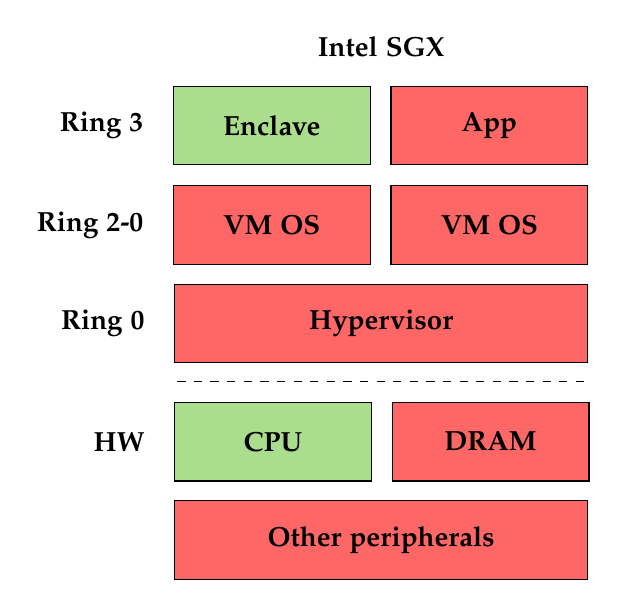
\begin{tikzpicture}

    % Define colors
    \definecolor{greenblock}{rgb}{0.67, 0.87, 0.55} % Light green
    \definecolor{redblock}{rgb}{1, 0.4, 0.4}        % Light red

    % Ring 3
    \node[rectangle, draw, fill=greenblock, minimum width=2.5cm, minimum height=1cm] (enclave) {\textbf{Enclave}};
    \node[rectangle, draw, fill=redblock, minimum width=2.5cm, minimum height=1cm, right=0.25cm of enclave] (app) {\textbf{App}};

    % Ring 2-0
    \node[rectangle, draw, fill=redblock, minimum width=2.5cm, minimum height=1cm, below=0.25cm of enclave] (vm1) {\textbf{VM OS}};
    \node[rectangle, draw, fill=redblock, minimum width=2.5cm, minimum height=1cm, right=0.25cm of vm1] (vm2) {\textbf{VM OS}};

    % Ring 0
    \node[rectangle, draw, fill=redblock, minimum width=5.25cm, minimum height=1cm, below=1.25cm of vm2.east, anchor=east] (hypervisor) {\textbf{Hypervisor}};

    % Dashed line
    \draw[dashed, below=0.5cm of hypervisor,  minimum width=5.25cm] (-1.2, -3.25) -- (4.05, -3.25);

    % HW
    \node[rectangle, draw, fill=greenblock, minimum width=2.5cm, minimum height=1cm, below=1.5cm of hypervisor.west, anchor=west] (cpu) {\textbf{CPU}};
    \node[rectangle, draw, fill=redblock, minimum width=2.5cm, minimum height=1cm, right=0.25cm of cpu] (dram) {\textbf{DRAM}};
    \node[rectangle, draw, fill=redblock, minimum width=5.25cm, minimum height=1cm, below=1.25cm of cpu.west, anchor=west] (other) {\textbf{Other peripherals}};

    % Title
    \node[anchor=north, above=2.75cm of hypervisor] {\textbf{Intel SGX}};

    % Ring Labels
    \node[anchor=east,  left=0.25cm of enclave] {\textbf{Ring 3}};
    \node[anchor=east, left=0.25cm of vm1] {\textbf{Ring 2-0}};
    \node[anchor=east, left=0.25cm of hypervisor] {\textbf{Ring 0}};
    \node[anchor=east, left=0.25cm of cpu] {\textbf{HW}};
\end{tikzpicture}
    \caption{Intel SGX threat model: green components are trusted, red are untrusted.}
    \label{fig:threath-model-intelSGX}
\end{figure}

\section{Remote Attestation (RA)}
Remote Attestation (RA) is a process that allows one party to verify the integrity and authenticity of software and hardware running on a remote system. It involves generating cryptographic proofs that the code running in a TEE, such as an SGX enclave, is genuine and has not been tampered with. RA ensures that the remote system is in a trusted state before sensitive data or operations are entrusted to it. 

\subsection{Remote Attestation in Intel SGX}
Remote Attestation (RA) in the context of Intel SGX allows an enclave to prove its identity and integrity to a remote party, thereby establishing a secure and trusted communication channel.

\subsubsection{Process Overview}
The RA process involves generating a signed quote by a special enclave known as the Quoting Enclave. This quote is a cryptographic statement that includes information about the enclave's measurement, called \texttt{MRENCLAVE}, which corresponds to the enclave's identity. The measurement is performed by the Intel processor.

\subsubsection{Establishing Secure Communication}
This mechanism ensures that sensitive operations and data exchanges are only conducted with trusted enclaves. Public keys or other data can be securely shared as part of the signed quote. Secure communication between enclaves on the same platform is achieved via local attestation.

\subsubsection{Verification by the Client} \label{sec:verification-client}
The client intending to verify the enclave's identity receives the quote. It first checks whether \texttt{MRENCLAVE} matches the expected value. The client then sends the quote to a remote attestation service, such as the Intel Attestation Service (IAS), for verification. Once the IAS verifies the quote, it provides a signed attestation report that confirms the enclave's authenticity and integrity.

The Intel Attestation Service (IAS) is a cloud-based service provided by Intel that facilitates remote attestation for SGX enclaves. The IAS acts as a trusted third party that verifies the quotes generated by SGX enclaves during the attestation process. It signs the attestation reports with its own Root Certificate Authority (CA).

\subsubsection{Remote Attestation over TLS} 
In \cite{sgx-ra-tls-white-paper}, Remote Attestation (RA) is integrated directly into the TLS protocol. In the proposed design, the enclave itself carries out the verification steps outlined in Section \ref{sec:verification-client}. The key idea is that the enclave retrieves the signed attestation report and provides it to the user, thereby eliminating the need for the user to directly contact the Intel Attestation Service (IAS).

The certificate used by the enclave during the TLS handshake includes, in its extensions section, both the quote and the corresponding signed attestation report. The client can verify this quote using the attestation report. The quote contains not only the identity of the enclave but also the public key corresponding to the private key used to sign the TLS certificate. This final step securely binds the identity of the enclave to the TLS certificate being used.



\chapter{System Model \& Requirements}\label{ch:sample-chapter}
This section outlines the key components of the system model and the associated requirements. The model is based on several critical assumptions and trust relationships, as detailed below.

\section{System Model}
Figure \ref{fig:communication-flow} illustrates an overview of the system model. The model consists of four distinct actors:
\begin{itemize}
    \item \textbf{Client:} The entity that wishes to visit a website via the web proxy hosted within the enclave.
    \item \textbf{Enclave:} A piece of code operating within an isolated execution environment, provided by Trusted Execution Environment (TEE) technology.    
    \item \textbf{Host:} The hardware and software infrastructure on which the Enclave is executed.
    \item \textbf{Backend:} The server that hosts the website the Client aims to access.
\end{itemize}

\begin{figure}[h!]
    \centering
    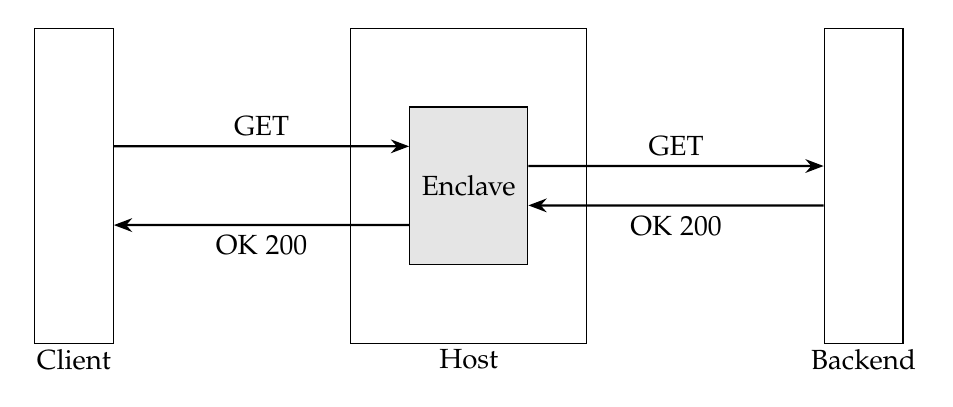
\begin{tikzpicture}[
        node distance=3cm,
        mynode/.style={draw, align=center, minimum height=4cm, minimum width=1cm},
        host/.style={draw, align=center, minimum height=4cm, minimum width=3cm},
        enclave/.style={draw, rectangle, minimum height=2cm, minimum width=1.5cm, fill=gray!20},
        arrow/.style={-Stealth, thick},
        adversary/.style={shape=diamond, draw=red, fill=red!30, minimum size=0.8cm, inner sep=0pt, label=above:{Adversary}}
    ]

    % Nodes
    \node [mynode] (client) {};
    \node [host](server) [right=of client] {};
    \node [mynode](backend) [right=of server] {};
    \node [mynode] (enclave) [enclave, above=1cm of server.south] {Enclave};

    % Labels
    \node at ([yshift=-0.2cm]client.south) {Client};
    \node at ([yshift=-0.2cm]server.south) {Host};
    \node at ([yshift=-0.2cm]backend.south) {Backend};

    % Arrows
    \draw[arrow] ([yshift=0.5cm]client.east) -- ([yshift=0.5cm]enclave.west) node[midway, above] {GET};
    \draw[arrow] ([yshift=-0.5cm]enclave.west) -- ([yshift=-0.5cm]client.east) node[midway, below] {OK 200};

    \draw[arrow] ([yshift=0.25cm]enclave.east) -- ([yshift=0.25cm]backend.west) node[midway, above] {GET};
    \draw[arrow] ([yshift=-0.25cm]backend.west) -- ([yshift=-0.25cm]enclave.east) node[midway, below] {OK 200};

    \end{tikzpicture}
    \caption{Example of communication flow between the Client, Enclave, and Backend server.}
    \label{fig:communication-flow}
\end{figure}


\section{Threat Model} \label{sec:threat-model}

As represented in Figure \ref{fig:threath-model}, the system adopts the Dolev-Yao model to describe the network adversary. In this model, the adversary not only monitors network traffic but also actively interferes with and tampers with messages. This capability includes intercepting, altering, and injecting messages into the network, which poses significant risks to data integrity and confidentiality. Additionally, it is assumed that the web proxy service operator is malicious, potentially exploiting their position to compromise the security of the hosted services or data. 

Additionally, it is assumed that it is not in the interest of a malicious host or network adversary to just prevent any communication between client, enclave and backend, i.e. the host could simply drop all the packets from/to the enclave.

\begin{figure}[h!]
    \centering
    \definecolor{redblock}{rgb}{1, 0.4, 0.4}
    \begin{tikzpicture}[
        node distance=3cm,
        mynode/.style={draw, align=center, minimum height=4cm, minimum width=1cm},
        host/.style={draw, align=center, minimum height=4cm, minimum width=3cm},
        enclave/.style={draw, rectangle, minimum height=2cm, minimum width=1.5cm, fill=gray!20},
        arrow/.style={-Stealth, thick},
        adversary/.style={shape=diamond, draw=black, fill=redblock, minimum size=0.8cm, inner sep=0pt, label=above:{Adversary}}
    ]

    % Nodes
    \node [mynode] (client) {};
    \node [host, fill=redblock](server) [right=of client] {};
    \node [mynode](backend) [right=of server] {};
    \node [mynode] (enclave) [enclave, above=1cm of server.south] {Enclave};

    % Labels
    \node at ([yshift=-0.2cm]client.south) {Client};
    \node at ([yshift=-0.2cm]server.south) {Host};
    \node at ([yshift=-0.2cm]backend.south) {Backend};
    
    % Adversary symbols (diamond shape)
    \node [adversary, yshift=2cm]  (adv1) at ($(client.east)!0.5!(server.west)$) {};
    \node [adversary, yshift=2cm] (adv2) at ($(server.east)!0.5!(backend.west)$) {};

    % Arrows
    \draw[arrow] ([yshift=0.5cm]client.east) -- ([yshift=0.5cm]enclave.west) node[midway, above] {GET};
    \draw[arrow] ([yshift=-0.5cm]enclave.west) -- ([yshift=-0.5cm]client.east) node[midway, below] {OK 200};

    \draw[arrow] ([yshift=0.25cm]enclave.east) -- ([yshift=0.25cm]backend.west) node[midway, above] {GET};
    \draw[arrow] ([yshift=-0.25cm]backend.west) -- ([yshift=-0.25cm]enclave.east) node[midway, below] {OK 200};

    \end{tikzpicture}
    \caption{Threat model.}
    \label{fig:threath-model}
\end{figure}

\section{Assumptions} \label{sec:assumptions}
\subsection{Trust Assumptions}

It is assumed that TEE technologies are secure and reliable, and mechanisms are provided for clients to verify remote TEE parties integrity. This level of trust is fundamental to the model and affects the security assurances that can be provided.

It is important to report that TEE technologies in reality are not perfect and present vulnerabilities. In the specific case of Intel SGX many vulnerabilities have been found as reported in this survey \cite{nilsson2020surveypublishedattacksintel}. It is not in the scope of this project to protect against these vulnerabilities.

Public Key Infrastructure (PKI) \cite{rfc5280} is also trusted for authentication during TLS handshakes.

\subsection{Client and Website Assumptions}

In this report, it is assumed that both the clients and the website's backends are not malicious. We do not protect the clients from websites served by backends that are vulnerable to XSS/CORS attacks. However, we must carefully design the proposed system so that it does not introduce additional XSS/CORS attacks.

\section{Requirements}
\subsection{Functional Requirements}
The goal is to develop an enclave that hosts a web proxy service. This service will function like a typical website, accessible through any browser or client. Users will be able to connect to and browse any website via this service. 

Specifically, a client sends a request to the enclave, specifying the resource of a website they wish to access. The enclave performs this request on behalf of the client contacting the specified website, including all headers, parameters, and body sent with the original request. The enclave then responds to the client with the requested resources, applying URL rewriting to ensure smooth navigation through the website always via the web proxy. Via URL rewriting all the URLs will now point to the web proxy instead of the external websites.

An example of the communication flow is illustrated in Figure \ref{fig:communication-flow}.

For instance, if the web proxy service is available at \texttt{proxy.com}, a user accessing \texttt{proxy.com} via their browser should be able to visit and interact with \texttt{ethz.ch} while remaining connected to \texttt{proxy.com}. In other words, even though the user is browsing \texttt{ethz.ch}, the browser should indicate that the connection is still to \texttt{proxy.com}.

\subsection{Security Requirements}
The security requirements of the model aim to ensure client privacy, meaning it should not be possible to determine which website the client is accessing through the web proxy service. Additionally, the communication between the client and the enclave, as well as between the enclave and the server, must satisfy the following properties: confidentiality and integrity. Furthermore, it is necessary for the client to authenticate the enclave and verify its identity, while the enclave must be able to authenticate the backend server.

Furthermore, all communication between the client and the target website, including any resources linked by the target website, must be routed through the enclave. For instance, on the line of the previous example, the user's browser should never communicate directly with \texttt{ethz.ch}. Failing to meet this requirement could compromise client privacy, as direct access to the target website would bypass the enclave.
\chapter{Design}\label{ch:sample-chapter}
The design of a secure web web proxy service was influenced by the need for a highly secure, yet flexible solution that is not tied to a specific platform. Instead of structuring the design around existing open-source proxies or web servers, the decision was made to design the web proxy service from scratch, allowing for complete control over security and performance. This section outlines the key design decisions.

\section{Enclave Design Decisions}
\subsection{Stream-based Data Forwarding} \label{stream-based-design}

Considering that the enclave has very limited memory, the design of the proposed web proxy service was made stateless. 

This means the service acts as a simple relay, just passing along packets without keeping track of who sent them or storing any data. This approach makes it easier to scale the service to handle more users.

Moreover, when a client makes a request, the service doesn’t wait to download the entire content from the backend before sending it to the client. Instead, it uses a streaming approach, where it downloads small chunks of data, for instance 4096 bytes at a time, and immediately sends them to the client. This way, the service uses much less memory.

\subsection{Fetching Resources via Enclave}
The structure of the path for a request to the web proxy service to fetch a remote resource is as follows:

\begin{quote}
\texttt{<enclave\_domain>?url=<backend\_url>}
\end{quote}

In this structure:
\begin{itemize}
    \item \texttt{<enclave\_domain>} is the domain of the web proxy service within the enclave.
    \item \texttt{<backend\_url>} is the full URL of the resource the client wants to fetch from a backend, specified in the \texttt{url} query parameter.
\end{itemize}

The \texttt{<backend\_url>} provided in the query parameter is used by the enclave to perform the actual request to a backend web server on behalf of the client. The request will also use the same HTTP method, headers, and body as the original request made to the service.


\subsection{URL rewriting} \label{sec:url-rewriting}
The content downloaded from the backend, whether it's HTML, CSS, or other types, will usually contain links to additional resources. If these links are not rewritten, the user's browser will directly connect to those resources when fetching them or when the user clicks on a link. A direct connection between the user's browser and the backend server will be visible to a network observer and will potentially leak information regarding the website the user is navigating to.

To ensure that all resources are accessed through the enclave, URLs are rewritten according to the following rule:

\texttt{<modified\_original\_domain>.<enclave\_domain>:<port>/?url=<original\_url>}

In this rule:
\begin{itemize}
    \item \texttt{<modified\_original\_domain>} corresponds to the original domain with all dots replaced by hyphens. For instance \texttt{sub.example.com} becomes \texttt{sub-example-com}. 
    \item \texttt{<enclave\_domain>} is the domain of the web proxy service running in the enclave.
    \item \texttt{<port>} is the port number used by the service (if needed).
    \item \texttt{<original\_url>} is the complete URL of the resource that needs to be fetched.
\end{itemize}

The original domain is prepended to the enclave domain in order to allow user's browser to enforce SOP (Same Origin Policy) across the different resources.

\subsection{Connection between Client, Enclave and Backend Server}
To protect the data exchanged over the network from any adversary and to secure all data going to and from the enclave, including from the host operating system, TLS (Transport Layer Security) is used. TLS ensures the confidentiality, integrity, and authenticity of the data.

When clients use the enclave service, they establish a TLS tunnel directly between themselves and the enclave. Similarly, when the enclave establishes a connection with a backend, it also uses TLS, if supported by the backend server.

Clients of the web proxy service will need to verify the enclave certificate using the mechanism described in Section \ref{sec:ra-over-tls}. Their root of trust will then be the TEE manufacturer, based on the TEE technology that was chosen.

\subsection{One thread per request}
To simplify the design, the current approach creates a new thread for each HTTPS request made by the client. Each thread handles the request by contacting the backend, processing it, and then terminating.

However, this design has a drawback: it initiates a new TLS handshake for every request. An improved approach would involve maintaining a persistent TLS connection throughout the duration of multiple requests. While this would reduce the overhead of repeated handshakes, it introduces additional complexity, such as managing and preserving TLS sessions and determining when a TLS connection can be safely closed.

\subsection{Remote Attestation during with TLS Handshake} \label{sec:ra-over-tls}
In a typical Trusted Execution Environment (TEE) setup, Remote Attestation (RA) is explicitly performed by the client. When a client connects to an enclave, it initiates a protocol to conduct the RA.
The challenge, in the context of this project, is that the client would first need to perform RA, receive a secret during the RA process, and then use that secret to establish secure communication with the enclave. While these steps are technically feasible, they would require the development of a specialized client. Moreover, all potential users of this service would need to download and use this special client, which would create significant overhead.

The goal is to make the user experience as seamless as possible, resembling normal navigation on a target website without requiring the use of a specialized client for the web proxy service.

To achieve this, in our design we use the solution proposed in this paper \cite{sgx-ra-tls-white-paper} which integrates RA with the standard TLS handshake, offering an ideal solution. The concept of RA-TLS allows the enclave to use a self-signed certificate during the TLS handshake. This self-signed certificate is signed with a key pair that can be verified with the RA report included in the certificate. The RA report can be verified with the TEE provider's Root CA, and it also contains the identity of the enclave. Thus, a client just needs to trust the TEE provider's  Root CA and can then verify locally the whole chain of trust and at the same time validate the identity of the enclave and the TLS handshake.

Practically speaking, a user can connect to the web proxy website hosted on the enclave just like they would with any other website. The client can manually check the certificate and RA report or use a tool like a browser extension for verification.

\subsection{SNI encryption} \label{sec:sni-encryption}
Due to the way URL rewriting is performed, the original website domain is fully included in the domain sent by the clients during TLS handshake.

In order to avoid leaking this information to a potential observer, Encrypted SNI (ESNI)\cite{esni} is leveraged. A public key is associated to the DNS record of the web proxy service. The client can then use the public key to encrypt its SNI record in such a way that only the enclave can decrypt it.

SNI encryption is also used during the TLS handshake with the backend when supported.

It is important to report that there exists also an alternative technology to solve the same problem: Encrypted Client Hello (ECH)\cite{ech}.

\subsection{Wildcard certificate and DNS records}
Thanks to the way URL rewriting is performed, potentially infinite subdomains can be used. To minimize the need for numerous certificates and DNS records, the following strategies are incorporated into the design.

For certificates, a wildcard certificate for \texttt{*.<enclave\_domain>} is issued, matching all the first level subdomains, as specified in \cite{rfc9525}.

For DNS, a wildcard DNS is employed, enabling a single entry to match all possible subdomains.

\subsection{DNS and Privacy Considerations}
A critical aspect to consider is the handling of DNS queries by the enclave, which are necessary for resolving the IP address of the server and retrieving the public key associated with the domain for Server Name Indication (SNI) encryption. Therefore, DNS queries must ensure confidentiality, integrity, and authentication of the endpoint being contacted.

This problem is well-documented, with established solutions such as DNS over TLS (DoT) \cite{rfc7858} or DNS over HTTPS (DoH) \cite{rfc8484} and a solution based on TEEs such as Private DNS-over-TLS (PDoT) \cite{Nakatsuka_2019} available. Determining the most suitable solution for this project is beyond its current scope.


\chapter{Implementation}\label{ch:sample-chapter}
\section{Development Environment}

\subsection{Tools and Technologies} \label{sec:tools-and-technologies}
We decided to implement the web proxy service with Intel SGX. The decision was influenced mainly by the previous knowledge of the technology by me and by the fact that Yoshimichi had already developed similar projects with Intel SGX. 

Intel-related technologies and corresponding versions:
\begin{itemize}
    \item \textbf{Intel SGX Version:} 2.4
    \item \textbf{Intel Attestation Service via EPID \cite{intelSGXattesationservice} API Version:} 5
\end{itemize}

The development and testing phases were carried out on a server provided by the System Security Group at ETH Zurich.

The server specifications are as follows:
\begin{itemize}
    \item \textbf{Operating System:} Ubuntu 20.04.6 LTS x86\_64
    \item \textbf{Kernel:} 5.4.0-97-generic
    \item \textbf{CPU:} Intel Pentium Silver J5005 (4 cores @ 1.500GHz)
    \item \textbf{Memory:} 5218 MiB
    \item \textbf{Enclave Page Cache (EPC) Size:} 128 MB
\end{itemize}

To ensure a stable and consistent environment for developing the web proxy service, the development and testing was carried in a Docker container running Ubuntu 18.04. This specific Ubuntu version was selected to ensure full compatibility with the Intel sgx-ra-tls library later described.

The development was done in C and the build is done via Makefiles. The choice of the programming language was highly influenced by the previous knowledge of the language compared to other choices such as Rust or C++ and, more significantly, by the amount of other Intel SGX Enclave projects that can be found online written using the same language. 

\subsection{Setting Up the Environment}
The environment setup process is documented in the codebase README.

Note that the remote attestation mechanism used in this project relies on Intel® SGX Attestation Service using Enhanced Privacy ID (EPID)\cite{johnson2016intel}. However, this service is scheduled for discontinuation: Development Access will be terminated on September 29, 2024, and Production Access on April 2, 2025, as detailed in this communication \cite{intelSGX-IAS-EOL}. 

Nevertheless, the library used in this project also supports Data Center Attestation Primitives (DCAP)\cite{dcap}, another attestation mechanism for Intel SGX, which will remain available and is not affected by this discontinuation.

\section{Custom Proxy Instead of Existing Solutions}
At the beginning of the project, using an open-source proxy or web server implementations was considered. However, it turned out that modifying these existing solutions to fit our specific design would be too complicated and time-consuming. So, it was decided that building a custom proxy from scratch would be easier and better suited to the project's needs.

\subsection{Proof of Concept Using Libraries}
Before engaging in the complex task of direct development with Intel SGX, we first assessed the feasibility of the approach using an integration layer: Gramine \cite{gramine}. This initial phase aimed to achieve two objectives: first, to determine if it was possible to fetch a website from within an enclave and serve it to users seamlessly, and second, to evaluate whether the enclave could support this operation with minimal overhead.

Gramine is described as a lightweight guest OS designed to run a single Linux application with minimal host requirements \cite{gramine}. By leveraging Gramine, it was possible to use the libraries \texttt{libhttpd} and \texttt{libcurl} within the enclave without any change to the library themselves. After resolving issues with the \texttt{manifest.template} file to mount necessary files for domain resolution and HTTPS requests, these libraries performed as expected. Thanks to these two libraries, it was possible to develop a basic web proxy service with just over 100 lines of code. This service uses HTTP to communicate to the clients and HTTPS to communicate to HTTPS-abled backend servers. 

\subsection{Challenges with Libraries Integration}
Intel SGX enclaves are isolated from the host operating system and do not have direct access to system calls. This isolation enhances security by preventing enclaves from performing privileged operations directly through the system call interface, thereby protecting against potential rogue OS interactions.

The above implementation leverages two libraries that do not work directly in an Intel SGX enclave due to their dependence on syscalls. In order to fix this issue and make the libraries working it is needed to define all the required system calls inside the enclave. The system calls can be provided with two strategies: by callings corresponding OCALLs or by implementing them direclty within the enclave, when possible.
Another factor to keep in mind is the complexity and size of these libraries, as well as the unclear internal logic of their functions. Modifying their underlying mechanisms to support a stream-based approach would be highly challenging.

Consequently, to maintain control over all the underlying logic and avoid excessive effort, it was decided to avoid the use of these two libraries in the final implementation.

\subsection{Using sgx-ra-tls library}
At this stage, developing a functional Intel SGX-based web proxy solution appeared to require manual implementation of several components: socket connections establishment, TLS handshakes with Remote Attestation (RA), HTTP protocol handling, and web proxy functionality. As a reader can probably tell, implementing these protocols from scratch, particularly TLS with RA, would be exceedingly difficult and time-consuming.

Therefore we decided to base the web proxy off of the \texttt{sgx-ra-tls} library \cite{sgx-ra-tls}. This library is an implementation of  an integration of Intel SGX Remote Attestation into the TLS connection setup. This library provides three implementations based on SSL libraries: wolfSSL, mbedtls, and OpenSSL.

The implementation based on wolfSSL was picked due to the fact that the library comes with an example of client and server applications written in C using the wolfSSL implementation. This implementation supports both IAS and DCAP Remote Attestation and constitutes a perfect base to develop an enclave supporting RA-TLS in Intel SGX. 

It is important to report that this library has been discontinued since December 20, 2022. Due to the lack of alternative open-source libraries integrating RA with TLS for Intel SGX and thanks to the fact that this library still works correctly, it was decided to go forward with it.
In order to avoid compatibility issues, it was made sure that the development environment versions used were the same that were lastly supported by the library. The versions are reported in Section \ref{sec:tools-and-technologies}.

\subsection{IAS instead of DCAP}
We decided to use IAS instead of DCAP, despite IAS being scheduled for deprecation as reported in \cite{intelSGX-IAS-EOL}. This decision was influenced by the simpler setup process for IAS, which can be completed in a few minutes compared to the more complex setup required for DCAP. The property of performing RA over TLS remains almost the same from a client perspective regardless of the choice between IAS and DCAP. Simplifying, the only difference is that with IAS there is one single root CA to be used to verify the report signature, while with DCAP, there is not a single root certificate, but different certificates could be used for different enclaves.

\section{Implementation Details}

\subsection{Enclave functionality via OCALLs or ECALLs}
The implementation of the service functionality inside the enclave can be approached in two ways (or a mixture of the two): either by performing all operations in the untrusted environment and only invoking the Enclave for sensitive operations via ECALLs, or by having the Enclave manage everything, using OCALLs only when system calls are necessary.

No matter the apporach, the number of ECALLs/OCALLs needs to be minimized for better performance. Therefore, the number of ECALLs and OCALLs would be the same regardless of the approach. It was decided to opt for the latter design (many OCALLs): this approach ensures that the Enclave maintains full control over the workflow, minimizing the exposure of ECALLs to the potentially malicious untrusted environment.

\subsection{Stream-based Data Forwarding and URL-rewriting}
The data forwarding mechanism is implemented as follows:

\begin{itemize}
    \item \textbf{From client to backend server:} The client's request is first fully received by the enclave before taking any action. This was not implemented in a stream-based fashion because the enclave needs to determine how to handle the request---whether to serve the welcome page or forward it to the backend server. In the latter case, the full URL must be constructed or retrieved before processing.
    
    \item \textbf{From backend server to client:} Responses are forwarded chunk by chunk as they are received, with URLs rewritten as needed. A chunk is defined as an arbitrary number of bytes, in the current implementation 4096 bytes, and correspond to the buffer used to receive data from the backend.
\end{itemize}

The URL rewriting is implemented similarly to what is described in the design section. The only difference is that the \texttt{modified\_original\_domain} of the rewritten URL is not modified, e.g., \texttt{sub.example.com} does not get modified and it will be used as it is, with the dots. 

Developing the URL rewriting algorithm was particularly challenging. Given the potential impact of URL rewriting on the web proxy service's performance, the algorithm was designed keeping efficiency in mind.

\subsubsection{Handling Split Tags Across Chunks}
One of the main challenges in developing this algorithm was ensuring it could handle cases where a tag begins in one chunk and ends in the next, or where the start of a tag itself is split across two chunks. To address this, the URL rewriting function takes both the current chunk and the next chunk in the stream as input. In situations like these, the next chunk is used to complete the URL rewriting. Although the algorithm does not rewrite URLs that span more than two chunks, this should not be common, given a chunk size of, for instance, 4096 bytes.

\subsubsection{Efficient Chunk Scanning for Performance}
Another challenge was designing the algorithm to be efficient. The core functionality involves scanning each chunk to be rewritten. For every opening tag (e.g., \texttt{href="}), the algorithm locates the corresponding closing tag (e.g., \texttt{"}) and rewrites the content between them according to the URL rewriting rules outlined in the previous chapter. The efficiency of this process was carefully considered, for instance by avoiding scanning the chunk multiple times.

\subsection{UX}
I kept the user experience (UX) of the implemented web proxy intentionally minimal. Upon connecting to the web proxy, the user is presented with a simple interface featuring a form where they can submit the URL they wish to visit, as shown in Figure \ref{fig:homepage}.

The web proxy navigation is designed to be as transparent to the user as possible as shown in \ref{fig:website-navigation}. This is possible thanks to the fact that the enclave does not inject any custom HTML into the visited pages. The only indication that the user is navigating through the web proxy is in the browser's address bar, where the connection to the web proxy is visible.

\begin{figure}[h!]
    \centering
    \includegraphics[width=1\linewidth]{media/homepage.png}
    \caption{Homepage of the web proxy.}
    \label{fig:homepage}
\end{figure}

\begin{figure}[h!]
    \centering
    \includegraphics[width=1\linewidth]{media/website-navigation.png}
    \caption{ETH website visited through the web proxy.}
    \label{fig:website-navigation}
\end{figure}

\subsection{Certificates Verification and Datetime inside the Enclave}
Root certificate pinning is implemented in the enclave to store the Root Certificate Authorities (CAs) needed to verify backend certificates. This is the fastest way to provide an enclave with the necessary Root CAs. An alternative method would be to set up a more complex mechanism to fetch Root CAs from a trusted source, which would allow the storage of only one certificate (to verify this source). However, this approach could create a single point of failure.

During the development phase, a significant amount of time was spent troubleshooting the persistent failures of TLS handshakes between the enclave and external servers. The root cause was eventually identified in the enclave not having the correct date, which led to certificates being deemed ``too new'' and therefore invalid. Securely obtaining the current time within an Intel SGX enclave is challenging due to its limited access to external resources, including system clocks. The primary difficulty lies in ensuring that the time source is trustworthy and immune to tampering, especially since enclaves operate in an untrusted environment.

Addressing this issue is complex and falls outside the scope of this project. As a temporary workaround, the date is currently hardcoded into the enclave's code.

\subsection{Enclave Certificate}
During the initialization phase, the enclave undergoes the Remote Attestation process via the Intel Attestation Service (IAS) and generates a self-signed certificate. This certificate includes the IAS report and its signature, which are used to verify the enclave's identity (MRENCLAVE). The IAS report binds the enclave's public key to its identity, and this binding can be validated using the Intel Root CA and the report signature. The public key is then used to self-sign the certificate, which will be used for all TLS connections between any client and the enclave.

\section{Browser Extension}

As previously discussed, the enclave uses a self-signed certificate. Consequently, when a user connects to the web proxy service via a browser, a warning is displayed indicating that the website is using a self-signed certificate. While it is theoretically possible for a user to manually verify the entire certificate chain and thus confirm the enclave's identity, this process requires significant time and expertise.

To address this issue, it was decided to developed a browser extension that automates the verification of the certificate chain used in the TLS connection between the browser and the enclave. The extension also clearly displays the enclave's identity (\texttt{MRENCLAVE}). However, is up to the user to check that the enclave's identity matches the expected value.

The simplified steps performed by the extension are as follows:
\begin{enumerate}
    \item Verify the signature of the report included in the TLS certificate using the Intel Root CA.
    \item Extract the public key from the report and compare it with the one used in the self-signed certificate.
    \item Extract and display the enclave's identity.
\end{enumerate}

The extension was developed for Firefox due to the browser's comprehensive developer tools, though it can be easily ported to other browsers. The source code is available in the project's codebase.

Figure \ref{fig:verified} shows the extension when verification is successful. In contrast, Figure \ref{fig:not-verified} shows the extension in the case of unsuccessful verification.

\begin{figure}[h!]
    \centering
    \includegraphics[width=1\linewidth]{media/verified.png}
    \caption{Successful verification of a certificate.}
    \label{fig:verified}
\end{figure}

\begin{figure}[h!]
    \centering
    \includegraphics[width=1\linewidth]{media/not-verified.png}
    \caption{Unsuccessful verification of a certificate.}
    \label{fig:not-verified}
\end{figure}

\clearpage
\section{Differences With Design} \label{sec:differences-with-design}
Beyond the minor differences with the design previously outlined in this section, there are additional key differences worth noting:
\begin{itemize}
    \item DNS queries are not performed using DoT\cite{rfc7858}, DoH\cite{rfc8484}, or PDoT\cite{Nakatsuka_2019}, as these are beyond the scope of the project and would add unnecessary complexity to the implementation.
    \item Only GET requests are supported, and client request headers are not utilized when making requests to the backend.
    \item SNI encryption is not supported on the client side and is not employed when making requests to the backend servers.
\end{itemize}

\chapter{Evaluation}\label{ch:sample-chapter}
\section{Security Analysis}
The following security analysis considers the two adversaries defined in Section \ref{sec:threat-model} and evaluates how the system design protects against these actors: a malicious host and a network adversary that intercepts communication between the client and the enclave, as well as between the enclave and the backend server.

\subsection{Malicious Host}
A malicious host controls the machine and operating system on which the enclave is running. Consequently, this adversary has full control over the data entering and exiting the enclave. Based on the trust model, the host may attempt the following actions:
\begin{itemize}
    \item tamper with messages
    \item impersonate the enclave
    \item impersonate a backend web server
    \item leak which website the client is connecting to
\end{itemize}


Regarding the first issue, the host is unable to tamper with messages because all communication to and from the enclave is conducted over TLS. TLS provides strong guarantees of confidentiality and integrity, ensuring that the host cannot successfully alter the messages and read their contents. Additionally, the use of TEE technology guarantees confidentiality and integrity of all the data inside the enclave. 

Typically, during a TLS handshake, the domain that the client expects to connect to is included in the first TLS message in plaintext. This could allow an adversary to determine which websites are being accessed, although they would not be able to view the actual data exchanged because of TLS confidentiality property. Our design mitigates this issue by supporting SNI encryption on the client side and utilizing SNI encryption when communicating with backend servers that support it.

For the second issue, the host cannot impersonate the enclave due to the remote attestation process performed over TLS. The host cannot produce a valid TLS certificate that includes a report signed by the remote attestation trusted authority (i.e., Intel) with the same identity (i.e., \texttt{MRENCLAVE}) as the genuine enclave. While a malicious host could create a rogue enclave capable of obtaining a certificate signed by trusted authority, the enclave identity included in the report would not match that of the trusted enclave because of the remote attestation protocol. Therefore, a client that verifies the enclave identity will not be deceived.

Regarding the third issue, we rely on authentication via TLS, using certificates verified through the PKI infrastructure. The enclave has hardcoded Root CAs that are used to verify the certificate received from the backend server. Thus, if the host attempts to impersonate a backend web server, it will be unable to provide a valid certificate corresponding to the accessed domain.

Finally, the fourth issue is addressed by the usage of TLS with ESNI and by the usage of a TEE. All these technologies provide confidentiality and do not leak any information to any observer. 

\subsection{Network Adversary}
A Dolev-Yao network attacker can intercept and tamper communication between the client and the enclave, as well as between the enclave and the backend server. In practice, a network attacker does not have more capabilities than a malicious host, as the host can also monitor and modify traffic like the network adversary. Therefore, since the design has been demonstrated to protect against a malicious host, it will also protect against a network adversary.

\subsection{Client-Side Security}

\subsubsection{Same Origin Policy}
It is assumed that neither clients nor the accessed websites are malicious, see Section \ref{sec:assumptions}. However, it is important to discuss the Same-Origin Policy (SOP).

Same-Origin Policy (SOP) \cite{rfc6454} is a fundamental security concept used in web browsers to restrict how documents or scripts loaded from one origin can interact with resources from another origin. This policy is designed to prevent malicious websites from accessing sensitive data from another site without any permission, thereby protecting users from various attacks, such as cross-site scripting (XSS) or cross-site request forgery (CSRF).

Thanks to the way URL rewriting is performed each website is translated into a unique subdomain, and thus perceived as distinct by the browser, allowing SOP to function correctly.

\subsection{Certificate and Report Validation}
To perform remote attestation successfully during the TLS handshake, the client requires two elements: the Root CA used for remote attestation (i.e., Intel SGX Root CA) and the identity of the enclave (i.e., MRENCLAVE).

The Root CA of the trusted authority can be downloaded from a trusted website. In the case of Intel, the Root CA can be downloaded over HTTPS from their website \cite{intelSGXattesationservice}. 

Regarding the enclave's identity, it can be obtained in one of two ways: via a trusted third party or by calculating it locally on a machine that supports the TEE technology used.

\section{Deployability}
\subsection{Enclave}
Deploying the proposed enclave implementation is straightforward. It only requires hardware that supports Intel SGX, after which all necessary dependencies can be installed to run the enclave without any particular issues. Besides deploying the enclave, it is also necessary to purchase a domain and configure DNS records to point to the enclave's host.

\subsection{Client}
On the client side, ideally, the browser would support Remote Attestation (RA) over TLS and include the trusted authority (i.e. Intel SGX Root CA) and automatically perform the steps handled by the proposed browser extension. Additionally, the browser should provide a way to verify the identity of the enclave, either automatically or manually.

Currently, browsers do not perform these tasks. However, it is still easy to navigate and use the enclave. The validity of the certificate and the identity of the enclave would need to be verified using additional tools, such as the proposed browser extension or manually.

\section{Performance Evaluation}

\subsection{Comparison with other Browsing Methods} \label{experiment-1}
\subsubsection{Objective}
The objective of this experiment is to compare the performance of browsing the internet using the proposed enclave-based system against normal browsing and browsing through a third-party web proxy tools.

\subsubsection{Setup}
\begin{itemize}
    \item \textbf{Environment}: 
    \begin{itemize}
        \item \textbf{Client:} All the experiments are run from a Linux laptop. The laptop is connected to internet via a stable wireless connection and is connected to ETH network via VPN (required to access the enclave). The websites are all accessed via Firefox version 128.0b9.
        \item \textbf{Enclave:} The enclave is running on the development machine described in Section \ref{sec:tools-and-technologies}. The enclave is reached from the client laptop via an SSH port forwarding. \\The enclave configuration is as follows:\\
        \texttt{<EnclaveConfiguration>\\
            <ProdID>0</ProdID>\\
            <ISVSVN>0</ISVSVN>\\
            <StackMaxSize>0x40000</StackMaxSize>\\
            <HeapMaxSize>0x1000000</HeapMaxSize>\\
            <TCSNum>100</TCSNum>\\
            <TCSPolicy>1</TCSPolicy>\\
            <DisableDebug>0</DisableDebug>\\
        </EnclaveConfiguration>}
        \item \textbf{Third-party web proxy tools:} The following two web proxies were selected as among the best performing. \texttt{proxysite.com} accordingly to \cite{similar-web} is the most used web proxy, but it performs badly compared to the following two.
        \begin{itemize}
            \item \texttt{genmirror.com}
            \item \texttt{de.hideproxy.me} 
        \end{itemize}
    \end{itemize}
    \item \textbf{Target Websites}: The experiment was conducted on two distinct websites to evaluate performance under different conditions:
    \begin{itemize}
        \item \texttt{syssec.ethz.ch}: Selected as a representative example of a typical webpage with a structured layout, including a header, body, and footer. It includes some CSS and JavaScript, though it does not depend on JavaScript for asynchronous content loading. The website also contains a large image file of 1.6 MB, contributing to an overall transferred size of slightly more than 3 MB.
        \item \texttt{example.com}: Chosen for its simplicity, serving as an example of a minimalistic website. It is a small, purely HTML-based site that does not load any additional resources beyond the main HTML file. The total transferred size is 1.04 KB.
    \end{itemize}
    \item \textbf{Metrics}: The following metrics are measured for each browsing method:
    \begin{itemize}
        \item \textbf{First Contentful Paint (FCP)\cite{w3-fcp}\cite{web-dev-fcp}}: FCP measures the time from when the user first navigated to the page to when any part of the page's content is rendered on the screen. 
        \item \textbf{Largest Contentful Paint (LCP)\cite{w3-lcp}\cite{web-dev-lcp}}: LCP reports the render time of the largest image, text block, or video visible in the viewport, relative to when the user first navigated to the page. Accordingly to \cite{w3-working-group} it is the best way to measure when the main content of a page has loaded.   
    \end{itemize}
\end{itemize}

\subsubsection{Procedure}
Each website is accessed with the following three methods:
\begin{enumerate}
    \item \textbf{Normal browsing}: The websites are accessed directly through Firefox.
    \item \textbf{Third-party web proxy tool}: The websites are accessed via \\\texttt{genmirror.com} and \texttt{de.hideproxy.me} from Firefox.
    \item \textbf{Enclave-based browsing}: The websites are accessed through the proposed enclave-based system from Firefox.
\end{enumerate}
For each condition, the above metrics are recorded via the Firefox Profiler tool \cite{firefox-profiler}: the metrics can be found under the \texttt{Marker Chart} section. The experiment is repeated 10 times for each method to ensure consistent results. Every time all the cache is invalidated in order to assure a full page reload.

\subsubsection{Results}
The table \ref{experiment1-table} summarizes the performance metrics obtained from the experiment. Each metric is averaged over 10 runs, and the standard deviation is calculated to assess the consistency of the results.

\begin{table}[h!] \label{experiment1-table}
\begin{center}
    \centering
    \caption{Performance Metrics for Different Browsing Methods Across Two Websites}
    \label{tab:performance_metrics}
    \begin{tabular}{lcccc}
        \toprule
        \textbf{Website} & \textbf{Method} & \textbf{Metric} & \textbf{Mean (ms)} & \textbf{Std. Dev. (ms)} \\
        \midrule
        \multirow{8}{*}{\centering \texttt{example.com}} 
            & \multirow{2}{*}{Normal Browsing} 
            & FCP & 568,70 & 62,83 \\
            & &  LCP & 574,50 & 62,86\\
            \cmidrule{2-5}
            & \multirow{2}{*}{\texttt{genmirror.com}} 
            & FCP & 702,40 & 60,42 \\
            & &  LCP & 710,40 & 60,71\\
            \cmidrule{2-5}
            & \multirow{2}{*}{\texttt{de.hideproxy.me}} 
            & FCP & 825,70 & 305,18 \\
            & &  LCP & 835,20 & 300,70\\
            \cmidrule{2-5}
            & \multirow{2}{*}{Enclave} 
            & FCP & 856,00 & 71,15 \\
            & &  LCP & 865,90 & 83,08\\
        \midrule
        \multirow{8}{*}{\centering \texttt{syssec.ethz.ch}} 
            & \multirow{2}{*}{Normal Browsing} 
            & FCP & 2370,80 & 540,98 \\
            & &  LCP & 2469,20 & 629,27\\
            \cmidrule{2-5}
            & \multirow{2}{*}{\texttt{genmirror.com}} 
            & FCP & 1078,10 & 346,63 \\
            & &  LCP & 1351,70 & 222,32\\
            \cmidrule{2-5}
            & \multirow{2}{*}{\texttt{de.hideproxy.me}} 
            & FCP & 1599,70 & 1358,73 \\
            & &  LCP & 2165,80 & 1712,12\\
            \cmidrule{2-5}
            & \multirow{2}{*}{Enclave} 
            & FCP & 7958,20 & 2052,89 \\
            & &  LCP & 10662,80 & 2393,69\\
        \bottomrule
        
    \end{tabular}
\end{center}
\end{table}

% \begin{figure}[h!] \label{experiment1-graph1}
%     \centering
%     \begin{tikzpicture}
%         \begin{axis}[
%             ybar,
%             symbolic x coords={Normal, Genmirror, HideProxy, Enclave},
%             xtick=data,
%             bar width=20pt,
%             ylabel={Time (ms)},
%             nodes near coords,
%             ymin=0,
%             legend style={at={(0.5,-0.15)}, anchor=north, legend columns=-1},
%             error bars/.cd, y dir=normal, y explicit,
%             enlarge x limits=0.3,
%             width=0.8\textwidth,
%         ]
%         \addplot+[
%             error bars/.cd,
%             y dir=both, y explicit,
%         ] coordinates {
%             (Normal, 150) +- (0,10)
%             (Genmirror, 180) +- (0,12)
%             (HideProxy, 170) +- (0,11)
%             (Enclave, 160) +- (0,11)
%         };
%         \addplot+[
%             error bars/.cd,
%             y dir=both, y explicit,
%         ] coordinates {
%             (Normal, 350) +- (0,15)
%             (Genmirror, 400) +- (0,20)
%             (HideProxy, 380) +- (0,18)
%             (Enclave, 370) +- (0,17)
%         };
%         \legend{First Content Time, Page Load Time}
%         \end{axis}
%     \end{tikzpicture}
%     \caption{Comparison of Performance Metrics across Different Browsing Methods for \texttt{www.ethz.ch}}
%     \label{fig:performance_comparison}
% \end{figure}
\clearpage
\subsubsection{Observations}
\begin{itemize}
    \item \textbf{FCP \& LCP}:
    \begin{itemize}
        \item \texttt{example.com}: The results show that all web proxies introduce a minor overhead of a few hundred milliseconds compared to non-enclave browsing. Despite this slight delay, the enclave demonstrates consistent response times comparing the standard deviation to other browsing methods. From a user experience perspective, browsing via the enclave does not significantly impact perceived performance.
        \item \texttt{syssec.ethz.ch}: For this website, there is a more noticeable disparity between enclave browsing and other methods. The load time difference—approximately 6 seconds for FCP and around 8 seconds for LCP—can likely be attributed to the enclave performing a TLS handshake for each resource fetched and to the delay introduced by the URL rewriting algorithm. Additionally, the enclave shows considerably higher instability, with a standard deviation of around 2 seconds for both metrics. It is also noteworthy that the two third-party web proxies outperform regular browsing. The reason for this probably comes from two factors: the fact that the third-party proxies do not load JavaScript resources and caching mechanisms employed by the proxies.
    \end{itemize}
    \item \textbf{Security Observations}: All resources loaded through the enclave and third-party web proxies are routed via the proxies themselves, with all URLs being correctly rewritten. A potential security concern is that the enclave allows users to fetch JavaScript resources, which could introduce risks. In contrast, the other two web proxies do not return any JavaScript, potentially reducing risk surface.
    \item \textbf{Content and Usability Observations}: The absence of JavaScript in the content loaded via the third-party web proxies impacts the user experience on \texttt{syssec.ethz.ch}: for instance, the navigation bar's menu does not function properly, whereas it works as expected in the Enclave. Additionally, both \texttt{genmirror.com} and \texttt{de.hideproxy.me} exhibit rendering issues with \texttt{example.com}. The first proxy overlays its navigation bar on the website content and displays empty white boxes below, while the second proxy fails to display any content, despite the content being present in the HTML code. The only notable drawback of the Enclave is the absence of a navigation bar for browsing to other websites.
\end{itemize}

\clearpage
\subsection{Load Testing of the Enclave Proxy} \label{experiment-2}
\subsubsection{Objective}
The objective of this experiment is to evaluate the scalability and performance of the enclave-based system under heavy load.

\subsubsection{Setup}
\begin{itemize}
    \item \textbf{Client:} All the experiments are run from a Linux laptop. The laptop is connected to internet via a stable wireless connection and is connected to ETH network via VPN (required to access the enclave). The websites are all accessed via Firefox version 128.0b9.
    \item \textbf{Enclave:} The enclave is running on the development machine described in Section \ref{sec:tools-and-technologies}. The enclave is reached from the client laptop via an SSH port forwarding. \\The enclave configuration is as follows:\\
    \texttt{<EnclaveConfiguration>\\
        <ProdID>0</ProdID>\\
        <ISVSVN>0</ISVSVN>\\
        <StackMaxSize>0x40000</StackMaxSize>\\
        <HeapMaxSize>0x1000000</HeapMaxSize>\\
        <TCSNum>100</TCSNum>\\
        <TCSPolicy>1</TCSPolicy>\\
        <DisableDebug>0</DisableDebug>\\
    </EnclaveConfiguration>}
    \item \textbf{Target Websites}: The experiment was conducted on two distinct websites to evaluate performance under different conditions:
    \begin{itemize}
        \item \texttt{syssec.ethz.ch}: Selected as representative of an average website. Its main HTML page size is 46.49 KB
        \item \texttt{example.com}: Chosen as a minimalist website with a very small HTML page size of 1.04 KB.
    \end{itemize}
    \item \textbf{Load Generation}: A Python script is used to generate an increasingly large number of requests to the enclave-based service to fetch the main HTML page of the target website.
    \item \textbf{Metrics}: The following metrics are recorded:
    \begin{itemize}
        \item \textbf{Response Time (ms)}: The time taken to respond to each request.
        \item \textbf{Failed clients}: The number of clients whose request failed for any reason. The timeout was set to 10 seconds.
    \end{itemize}
\end{itemize}

\subsubsection{Procedure}
The script generates a steadily increasing number of concurrent requests to the service (clients), starting from 5 increasing to 100 with an increment of 5. 100 is chosen as being the maximum amount of threads that can be spawned in the enclave (\texttt{TCSNum}). Metrics are recorded throughout the test.

\subsubsection{Results and Observations}
As shown in Table \ref{tab:experiment2-table}, the Enclave's average response time increases as the number of clients grows. Additionally, the standard deviation also rises with more clients, indicating that the Enclave's performance becomes less consistent across different clients.

The number of clients whose requests cannot be fulfilled is correlated with the total number of clients. It is noticeable that when the maximum amount of threads that can be spawned is almost reached, many client's requests start to fail. 

The difference in mean response times between \texttt{example.com} and \\\texttt{syssec.ethz.ch} is primarily due to the different page sizes and the additional overhead introduced by the URL rewriting algorithm.

It is insightful to also compare the average time required to load \\\texttt{syssec.ethz.ch} between the two experiments. In experiment 1 (Table \ref{experiment1-table}), loading the full 3MB page took roughly 8 seconds on average. In contrast, in experiment 2 (Table \ref{tab:experiment2-table}), loading only the main HTML file of 46 KB took about 5 seconds. This discrepancy can be attributed to the current implementation of the Enclave, where no URL rewriting is applied to JavaScript or image resources. Therefore, since most of the resources loaded after the main HTML page are of these types and account for most of the full page size, the additional URL rewriting overhead is minimal compared to the size left to load.


\begin{table}[h!]  \label{tab:experiment2-table}
\centering
\caption{Performance Evaluation of Web Proxy}
\begin{tabular}{lcccc}
\hline
\textbf{Website}        & \textbf{Clients} & \textbf{Mean (ms)} & \textbf{Std. Dev. (ms)} & \textbf{Failed} \\ \hline
\multirow{20}{*}{example.com} 
    & 5  & 791.30  & 15.50  & 0 \\ \cline{2-5} 
    & 10 & 854.74  & 25.70  & 0 \\ \cline{2-5} 
    & 15 & 929.94  & 15.96  & 0 \\ \cline{2-5} 
    & 20 & 992.51  & 77.49  & 0 \\ \cline{2-5} 
    & 25 & 1080.67 & 71.10  & 0 \\ \cline{2-5} 
    & 30 & 1149.33 & 59.64  & 0 \\ \cline{2-5} 
    & 35 & 1341.14 & 85.00  & 0 \\ \cline{2-5} 
    & 40 & 1408.64 & 46.34  & 1 \\ \cline{2-5} 
    & 45 & 1427.35 & 71.15  & 0 \\ \cline{2-5} 
    & 50 & 1546.80 & 52.87  & 1 \\ \cline{2-5} 
    & 55 & 1683.13 & 169.36 & 1 \\ \cline{2-5} 
    & 60 & 1817.31 & 70.88  & 5 \\ \cline{2-5} 
    & 65 & 1825.99 & 127.16 & 2 \\ \cline{2-5} 
    & 70 & 1883.74 & 86.34  & 2 \\ \cline{2-5} 
    & 75 & 2005.99 & 133.88 & 1 \\ \cline{2-5} 
    & 80 & 2171.65 & 154.28 & 1 \\ \cline{2-5} 
    & 85 & 2362.93 & 129.42 & 3 \\ \cline{2-5} 
    & 90 & 2517.20 & 166.87 & 8 \\ \cline{2-5} 
    & 95 & 2200.05 & 235.89 & 13 \\ \cline{2-5} 
    & 100 & 2276.80 & 152.29 & 23 \\ \hline
\multirow{20}{*}{syssec.ethz.ch} 
    & 5  & 5416.14  & 16.94  & 0 \\ \cline{2-5} 
    & 10 & 5479.61  & 19.13  & 0 \\ \cline{2-5} 
    & 15 & 5558.53  & 55.19  & 0 \\ \cline{2-5} 
    & 20 & 5642.45  & 46.91  & 0 \\ \cline{2-5} 
    & 25 & 5753.90  & 44.34  & 0 \\ \cline{2-5} 
    & 30 & 5928.72  & 29.45  & 0 \\ \cline{2-5} 
    & 35 & 6005.51  & 51.53  & 1 \\ \cline{2-5} 
    & 40 & 6092.17  & 155.80 & 0 \\ \cline{2-5} 
    & 45 & 6340.97  & 80.53  & 0 \\ \cline{2-5} 
    & 50 & 6429.52  & 129.35 & 3 \\ \cline{2-5} 
    & 55 & 6496.02  & 119.30 & 3 \\ \cline{2-5} 
    & 60 & 6628.77  & 174.67 & 0 \\ \cline{2-5} 
    & 65 & 6760.93  & 163.51 & 0 \\ \cline{2-5} 
    & 70 & 6823.51  & 221.77 & 0 \\ \cline{2-5} 
    & 75 & 6868.67  & 223.83 & 1 \\ \cline{2-5} 
    & 80 & 7157.64  & 329.74 & 0 \\ \cline{2-5} 
    & 85 & 7036.75  & 346.21 & 1 \\ \cline{2-5} 
    & 90 & 7226.61  & 276.04 & 0 \\ \cline{2-5} 
    & 95 & 7262.28  & 330.23 & 5 \\ \cline{2-5} 
    & 100 & 7392.69  & 219.73 & 10 \\ \hline
\end{tabular}
\end{table}




\chapter{Discussion}\label{ch:sample-chapter}
\section{Design Limitations and Considerations}

\subsection{Balancing performance and security for URL rewriting} \label{sec:url-rewriting-limitations}
URL rewriting ensures that when a client clicks a link within received web content, they continue navigating through the website via the web proxy and that the browser keeps loading resources via the web proxy. For purely HTML-based websites, it is feasible to rewrite all URLs to point to the enclave instead of the target site. However, modern websites often deliver content in various formats, such as JSON. To maintain consistent proxy navigation, the URL rewriting algorithm must be applied to all data passing through the enclave. Otherwise, some URLs might not be rewritten, leading the browser to load resources directly from the website's server, or allowing a user to click a link and navigate to the website without passing through the enclave.

This poses challenges because, unlike HTML, where URLs are clearly defined (e.g., in \texttt{<a>} tags with \texttt{href} attributes), identifying and rewriting URLs within JSON or other formats is complex and may result in a slower and more intricate algorithm. Additionally, handling dynamically generated URLs via JavaScript is particularly challenging. Since these URLs cannot be captured through static analysis, the enclave would need to execute the JavaScript locally and return the generated content statically. However, this approach is infeasible due to potential performance degradation and security risks, as it involves executing potentially malicious code within the enclave.

The most practical solution is to disable JavaScript or any mechanisms that allow dynamic URL creation, although this could significantly affect user experience.

Other web proxies address the challenge of balancing performance and security in various ways: some choose not to serve JavaScript files, while others employ faster URL algorithms that may not capture all URLs on the page.

\subsection{IP Leak, Anonymity Set, and Correlation Attacks} \label{sec:IP-leak}
While the IP addresses of the client and of the enclave do not directly reveal the websites being visited, the IP address of the backend server could potentially disclose the exact website or narrow it down to a small set of possibilities. This is because an IP address, in simplified terms, is associated with a server that may host one or more websites, and this information might be known to an attacker. For example, a popular website might be hosted on a server with a specific IP, making the accessed domain easily identifiable.

In such scenarios, maintaining client anonymity requires a large anonymity set (i.e., many clients using the service simultaneously), so it is not immediately obvious which client is accessing which server. However, even with a large anonymity set, privacy may not be fully guaranteed due to potential side-channel correlation attacks. An attacker monitoring both the connection between the client and the enclave and the connection between the enclave and the backend could match the request patterns on both sides, revealing the accessed website.

A possible mitigation is to introduce noise in the communication between the client and the enclave, as well as between the enclave and the backend.  This noise could involve random delays, dummy requests, or padding added to the data being transmitted, making it more difficult for an attacker to infer sensitive information based on timing or traffic patterns. However, this approach might not be effective against statistical side-channel attacks that analyze multiple traces over time.

While it is unlikely that an attacker would possess all the necessary knowledge about IP-to-domain mappings and the ability to monitor both network segments, the risk cannot be completely dismissed.

\subsection{Handling Non-SNI-Compliant Backends}
As discussed in Section \ref{sec:sni-encryption}, Encrypted Server Name Indication (ESNI) is leveraged to ensure the anonymity of the accessed website from attackers monitoring the connection between the client and the enclave. Although ESNI adoption is increasing, as of 2022, less than 20\% of websites use it \cite{SNI-adoption}. When ESNI is not supported, a network observer could identify the website being accessed by the enclave, making it easier to link the client to the website and compromising privacy.

\subsection{Fingerprinting Attacks} \label{sec:fingerprinting-attacks}
Section \ref{sec:IP-leak} describes a class of side-channel attacks where an attacker tries to match client requests with enclave requests to identify the accessed website. Another type of attacks involves website fingerprinting, where the sizes and patterns of requests are used to identify the website being accessed by a client.

To defend against such attacks, noise could be injected into the communication, such as extra packets or varying packet sizes. However, even with noise, statistical side-channel attacks could still succeed if sufficient data is collected.

A more robust solution would be to design a new protocol between the client and the enclave specifically to prevent these attacks. However, this is not be practical and will require custom clients making the proposed solution not accessible to most users.

\subsection{One New Thread Per Request} 
Each HTTP request from a client spawns a single thread, initiating a new TLS handshake. This introduces significant overhead. An improvement could involve maintaining an open session and reusing the established TLS session, though determining when to close the TLS connection and terminate the thread would be challenging.

\section{Implementation Limitations}
The following limitations of the current implementation, not covered in Section \ref{sec:differences-with-design}, are reported:
\begin{itemize}
    \item \textbf{Support for TLS-enabled Backends Only:} The current implementation only supports HTTPS backends, as the HTTP protocol is implemented on top of the TLS connection and cannot function independently over TCP.
    \item \textbf{Limited URL rewriting capabilities:} As explained in Section \ref{sec:url-rewriting-limitations}, it is very challenging to perform URL rewriting such that it captures all URLs present in a website. The algorithm currently implemented relies on tags to spot URLs, thus it cannot rewrite URLs in unstructured data and URLs dynamically generated.
    \item \textbf{No Support for Transfer-Encoding:} The web proxy does not support any HTTP Transfer-Encoding \cite{http-transfer-encoding}, resulting in an inability to load websites that rely on it, such as \texttt{google.com}.
    \item \textbf{TLS Version:} Only TLS 1.2 is supported by the proxy.
\end{itemize}

\section{Attack on SOP}
The current design of rewritten URLs effectively allows browsers to enforce SOP. However, cross-site scripting (XSS) or cross-site request forgery (CSRF) attacks could still be possible under specific conditions where it is possible to circumvent SOP.

As discussed in Section \ref{sec:url-rewriting}, a URL like \texttt{sub-to.example.com} is rewritten as \texttt{sub-to-example-com.<enclave\_domain>}. However, a different website, such as \texttt{sub.to-example.com}, would be rewritten to the same subdomain. An attacker could exploit this by crafting a malicious domain B that, when rewritten, corresponds to the same domain as target domain A, enabling XSS or CSRF attacks.

This attack requires that the target domain includes a hyphen in its name. A condition that is difficult to meet, as many domains do not have hyphens. Additionally, the malicious domain must be available for purchase.

An effective method to completely prevent such attacks is to use dots instead of hyphens when generating subdomains. For example, \texttt{sub-to.example.com} would be rewritten as \texttt{sub-to.example.com.<enclave\_domain>}. 

This approach, however, introduces significant challenges in certificate management when wildcard certificates are used. Wildcard certificates are valid only for single-level subdomains, meaning a certificate like \\ \texttt{*.<enclave\_domain>} would not cover deeper subdomains created through this method. Obtaining custom certificates for every possible website a customer might access is impractical and inefficient.

A feasible solution is to utilize certificates without a specified Common Name (\texttt{CN}), allowing them to be considered valid for any domain and subdomain. This would simplify certificate management and ensure secure connections across all dynamically generated subdomains.

Another approach could involve the replacement of the dots with different fixed strings relatively to the dot position. 


\chapter{Related Work}\label{ch:sample-chapter}
Various approaches have been developed in the field of internet privacy and security to protect user anonymity and secure online activities. This section reviews the related work on proxies, VPNs, Tor, and web proxy services, highlighting how the proposed approach differs from existing solutions and addresses the challenges identified in existing research.

\section{Alternative Solutions}
\subsection{Proxies}
Traditional proxy servers act as intermediaries between users and destination servers, forwarding requests and responses while hiding the user's IP address from the destination server. However, traffic between the client and the proxy lacks inherent security guarantees provided by the proxy itself; security is instead ensured by the protocol used between the client and the backend server. Proxies must be manually configured at the OS or browser level, and because they handle all traffic, a malicious proxy can see both the source and destination of the packets, gaining full knowledge of this information.

Web proxies differ in the sense that they are typically accessed via a web interface, requiring no manual configuration at the system level. Instead of managing all network traffic, web proxies handle only web traffic \\(HTTP/HTTPS), allowing users to access specific websites by entering the desired URL into the proxy's web interface. Unlike traditional proxies, which can obscure the user's IP address but expose the full range of their online activity, a web proxy's scope is limited to the websites users visit through the proxy service itself. The web proxies are more accessible but introduce risks, as users rely entirely on the proxy provider to securely handle their web traffic. The proxy service could potentially inspect, modify, or log the user’s web activity, leading to privacy concerns, especially when sensitive data is involved.

\subsection{Virtual Private Networks (VPNs)}
VPN technology establishes an encrypted tunnel between the user and the VPN server, through which all client-server communication is routed before exiting to the internet via the VPN server. While this method enhances privacy, it shares certain limitations with proxies: the VPN server has complete visibility into the traffic. Consequently, the server must be trusted; however, there is no assurance that it is trustworthy or that it refrains from collecting user data, as discussed in \cite{285411} and \cite{10.1145/3278532.3278570}.

Additionally, setting up a VPN requires extra software and technical expertise, making it less accessible to non-experts. On a typical laptop, setting up a VPN may involve downloading and installing new software or browser extensions. For non-tech-savvy users, this process may be challenging. More importantly, in environments with restricted privileges (i.e. public library computers) users may be unable to install necessary software or browser extensions thus they would not be able to use VPN at all.

Finally, VPNs can be blocked through techniques such as VPN fingerprinting \cite{280012} or IP blacklisting of known VPN servers.

\subsection{Tor}
The Tor network \cite{tor} is a decentralized system designed to anonymize users' internet activities by routing traffic through multiple volunteer-operated nodes. Each node only knows the preceding and following nodes, ensuring that no single entity can trace the entire path. Although Tor provides strong anonymity, its multi-hop design results in performance degradation. Moreover, Tor requires the use of a dedicated browser, which may not be easily accessible to inexperienced users. 

\subsection{Comparison with Proposed Solution}
The solution proposed in this project addresses the limitations identified above by offering a web-based proxy that is easily accessible via any browser without the need to install any extra software. Additionally, it provides a mechanism to verify the trustworthiness of the proxy through Remote Attestation (RA) and ensures that all communication between the client, enclave, and backend servers is encrypted via TLS. One issue this solution does not mitigate is correlation attacks, where an attacker observing both sides of the network could correlate client and enclave requests as discussed in Section \ref{sec:IP-leak}. Such attacks are partially \cite{evers2016thirteen} prevented by Tor thanks to the use of multiple relays.

\section{Web Proxy Services}
\subsection{Existing solutions}
There are numerous web proxy services available worldwide. According to \cite{similar-web}, some of the most widely used include:
\begin{itemize}
    \item \texttt{proxysite.com} \cite{proxy-site}
    \item \texttt{hide.me} \cite{hideme}
    \item \texttt{freeproxy.io} \cite{freeproxy}
    \item \texttt{genmirror.com} \cite{genmirror}
\end{itemize}

These proxies, however, present significant security issues as detailed in \cite{watanabe2020melting}. A primary concern is that all rehosted websites share the same origin (full domain), leading to most of the following vulnerabilities:
\begin{itemize}
    \item \textbf{Persistent MITM:} Web proxies act as full Man-In-The-Middle (MITM) entities since they can see all traffic between the client and backend servers unencrypted. They have the capability to manipulate, drop, or craft messages.
    \item \textbf{Session Hijacking and Injection:} Since all visited websites from the enclave share the same origin, an attacker can easily steal cookies from another website, facilitating session hijacking or injecting new cookies to force a victim to log into a specific account when visiting a target website.
    \item \textbf{Privilege Abuse:} Web pages sometimes request access to computer resources like cameras or microphones, which are associated with the origin. These permissions are then shared with all re-hosted websites and can be exploited by rogue websites.
    \item \textbf{Credential Theft:} Browser-stored credentials are associated with the origin, and in some cases, are autofilled in forms. A rogue website could steal credentials for other websites.
    \item \textbf{History Theft:} Many modern websites use cookies and local storage in the browser to store data. An attacker could monitor cookies and local storage with malicious scripts to determine which websites are visited via the web proxy. The feasibility of this technique for website fingerprinting is demonstrated in \cite{watanabe2020melting}.
    \item \textbf{Partial URL Rewriting:} It was observed that certain web proxies, such as \texttt{proxysite.com}, do not consistently rewrite all URLs in the resources they download. This results in the browser directly accessing remote resources without going through the proxy.
\end{itemize}

On the user experience side, during the course of this project, I observed inconsistent behavior by some proxies. For example, websites like \texttt{google.com} occasionally failed to load correctly.

\subsection{Comparison with Proposed Solution}
The proposed design addresses all the issues mentioned above. Regarding the MITM issue, RA allows the client to verify that the enclave is trustworthy and will behave as expected. The other vulnerabilities are mitigated by ensuring that all websites accessed via the web proxy correspond to different subdomains, thus preventing them from sharing the same origin. This effectively neutralizes the security concerns associated with existing web proxy solutions.
\chapter{Conclusion \& Future Work}\label{ch:sample-chapter}
\section{Conclusion}
This project has examined the design and implementation of a web-based proxy solution that addresses significant security and privacy challenges inherent in existing web proxies. The proposed service offers enhanced accessibility compared to VPNs and Tor-based solutions, while leveraging Trusted Execution Environments (TEEs) and Remote Attestation (RA) to ensure encrypted communication and authentication between the client, enclave, and backend servers. By employing RA and assigning different origins to different websites, the system effectively mitigates vulnerabilities commonly found in traditional web proxies, such as MITM attacks, session hijacking, privilege abuse, and credential theft. However, the solution still has limitations, particularly in defending against correlation attacks and traffic fingerprinting.

\section{Future Work}
While the proposed solution offers significant improvements over existing technologies, there are several areas for future research and development:
\begin{itemize}
    \item \textbf{Mitigation of Correlation and Fingerprinting Attacks:} Future research should focus on developing strategies to defend against correlation and fingerprinting attacks, potentially by integrating techniques from the Tor technology or exploring new cryptographic methods.
    \item \textbf{Performance Optimization:} The current implementation could benefit from optimizations to reduce overhead, particularly in high-traffic scenarios or when handling multiple concurrent connections.
    \item \textbf{Enhancing User Experience:} Improving the user interface and incorporating a seamless method for performing RA over TLS within browsers would make the system more user-friendly, promoting broader adoption.
\end{itemize}

In conclusion, this project has made significant progress in improving web proxy security, but ongoing research and development are essential to address remaining challenges and expand the system's capabilities and adoption.

% \appendix
% \input{appendix}

\backmatter

\bibliographystyle{plain}
\bibliography{refs}

\includepdf[pages={-}]{signed-declaration-originality.pdf}

\end{document}
